\section{The real simplex identity}\label{sec:simplex}

The lens boundary law now turns the feasibility sum into an exact
integral over the strip body. The simplices in this integral lie in the
polar body; their missing volume will also be the quantity used in the
equality argument.

Keep the nonzero spanning, pairwise nonproportional rows of
\eqref{eq:strip-body}. For $X\in\operatorname{int}A$, define
\begin{equation}\label{eq:real-feasibility-body}
 L_X=\{Y\in\R^d:|b_jY|\leq\lambda(b_jX)
                         \text{ for every }j\}.
\end{equation}
All widths are strictly positive, so $L_X$ contains a neighborhood of
$0$; a basis of rows shows that it is bounded. It is therefore a convex
polytope with nonempty interior.
For a basis $I$ and signs $\epsilon=(\epsilon_i)_{i\in I}\in\{-1,1\}^I$,
let
\[
 Y_{I,\epsilon}(X)=B_I^{-1}
          \bigl(\epsilon_i\lambda(b_iX)\bigr)_{i\in I}.
\]
We call $(I,\epsilon)$ feasible at $X$ when this vector belongs to $L_X$.
This definition specifies a unique vector for every choice, whether or
not it is feasible. Set
\begin{equation}\label{eq:feasible-simplex-union}
 T_{I,\epsilon}=\operatorname{conv}
                  \bigl(0,\{\epsilon_i b_i:i\in I\}\bigr),
 \qquad
 \Sigma_X=\bigcup_{(I,\epsilon)\text{ feasible at }X}T_{I,\epsilon}.
\end{equation}
Thus $\Sigma_X$ is a finite union of closed $d$-simplices contained in
$C=A^\circ$. This definition applies at every interior $X$, including
points with additional tight constraints. For integration only, declare
every pair infeasible and set $\Sigma_X=\varnothing$ when
$X\in\partial A$.

A feasible pair specifies a vertex $Y_{I,\epsilon}(X)$ of $L_X$.
A strictly positive combination of its signed tight rows defines a
linear functional maximized uniquely at that vertex. This is why
different feasible pairs give simplices with disjoint interiors
whenever their vertices are distinct. The proof below removes, outside
a null set of $X$, the boundary ties that could make two pairs specify
the same vertex.

\begin{proposition}[Feasible-simplex identity]\label{prop:simplex-integral}
Let $b_1,\ldots,b_m$ be nonzero, pairwise nonproportional real rows
spanning $(\R^d)^*$, and let $F,D,\lambda$ be as in
Lemma~\ref{lem:planar-lens}. With $A$, $S$, and $\Sigma_X$ defined in
\eqref{eq:strip-body}, \eqref{eq:feasible-probabilities}, and
\eqref{eq:feasible-simplex-union}, respectively,
\begin{equation}\label{eq:simplex-integral}
 1\leq S
   =\frac{d!}{4^d}\int_A|\Sigma_X|\,dX
   \leq\frac{d!}{4^d}|A|\,|A^\circ|.
\end{equation}
In particular, $|A|\,|A^\circ|\geq4^d/d!$, and
\begin{equation}\label{eq:simplex-deficit}
 0\leq\int_A\bigl(|A^\circ|-|\Sigma_X|\bigr)\,dX
       \leq |A|\,|A^\circ|-\frac{4^d}{d!}.
\end{equation}
\end{proposition}

\begin{proof}
We first convert each probability into a real integral. By
\eqref{eq:lens-boundary-law}, each active boundary coordinate has the
law $\epsilon_i\lambda(t_i)+it_i$, with $t_i$ uniform on $[-1,1]$ and
$\epsilon_i$ an independent fair sign. Consequently each fixed sign
choice has joint measure $4^{-d}\,dt_I$ on $[-1,1]^d$.
Writing the inferred complex vector as $Y+iX$ gives
\[
 t_I=B_IX,\qquad Y=Y_{I,\epsilon}(X).
\]
The constraints that all row coordinates lie in $\overline D$ are
exactly $X\in A$ and $Y\in L_X$, apart from the immaterial boundary
$\partial A$. This boundary has measure zero, since it is contained in
the finitely many hyperplanes $b_jX=\pm1$. The change of variables
$t_I=B_IX$ therefore gives
\begin{equation}\label{eq:probability-real-integral}
 P_I=\frac{D_I}{4^d}\int_A
       \sum_{\epsilon\in\{-1,1\}^I}
         \mathbf1\{(I,\epsilon)\text{ is feasible at }X\}\,dX.
\end{equation}

For almost every $X\in\operatorname{int}A$, every feasible pair
$(I,\epsilon)$ has no tight constraint outside $I$. Indeed, such an
additional equality means that an extra row of $Y+iX$ lies on
$\partial D$. Lemma~\ref{lem:boundary-ties} makes this event null in the
basis phases; the boundary law and the invertible change $t_I=B_IX$
make its set of $X$ null for each fixed sign choice. There are finitely
many bases, sign choices, and extra rows, so a single null set removes
all these equalities.

Fix $X$ outside this null set. Distinct feasible pairs have distinct
vectors $Y_{I,\epsilon}(X)$. If their bases differ, a shared vector would
have a tight row outside one of the bases. If their bases agree but
some signs differ, the shared vector would satisfy opposite equations
with the same strictly positive width, which is impossible.

The interiors of their simplices are disjoint. To see this, let
$e\in\operatorname{int}T_{I,\epsilon}$. It has a representation
$e=\sum_{i\in I}\alpha_i\epsilon_i b_i$ with all $\alpha_i>0$ and
$\sum_i\alpha_i<1$. For every $Y\in L_X$,
\[
 eY\leq\sum_{i\in I}\alpha_i\lambda(b_iX),
\]
and equality holds at $Y_{I,\epsilon}(X)$. Equality forces every
independent equation
$\epsilon_i b_iY=\lambda(b_iX)$, so this is the unique maximizer of the
linear functional $e$ on $L_X$. If $e$ belonged to the interiors of two
feasible simplices, their distinct vectors would both be its unique
maximizer, a contradiction.
Each simplex has volume $D_I/d!$, and their boundaries have measure
zero. It follows that, for almost every $X$,
\begin{equation}\label{eq:simplex-volume-sum}
 d!\,|\Sigma_X|
      =\sum_{I\in\mathcal B}\sum_{\epsilon\in\{-1,1\}^I}
               D_I\,\mathbf1\{(I,\epsilon)\text{ is feasible at }X\}.
\end{equation}

All integrals here are measurable. For each pair, feasibility is a
finite collection of closed inequalities between continuous functions
of $X\in\operatorname{int}A$. In particular the set
\[
 \{(X,e):X\in\operatorname{int}A,\ e\in\Sigma_X\}
\]
is a finite union of products of Borel feasibility sets and fixed
closed simplices. Fubini's theorem makes $X\mapsto|\Sigma_X|$
measurable, and it is bounded by $|C|$.
Sum \eqref{eq:probability-real-integral}, use
\eqref{eq:simplex-volume-sum}, and apply
Lemma~\ref{lem:holomorphic-feasibility}. This proves the first equality
and lower bound in \eqref{eq:simplex-integral}. The containment
$\Sigma_X\subset C$ proves the upper bound. In particular, the missing
volume has the exact expression
\[
 \int_A\bigl(|C|-|\Sigma_X|\bigr)\,dX
   =|A|\,|C|-\frac{4^d}{d!}S.
\]
It is nonnegative by containment, and $S\geq1$ bounds it above by
$|A|\,|C|-4^d/d!$. This proves \eqref{eq:simplex-deficit} and identifies
the quantity that will tend to zero in the equality argument.
\end{proof}

For a concrete union with positive missing volume, take
$b_1=(1,0)$, $b_2=(1/2,\sqrt3/2)$, $b_3=b_2-b_1$, and
$X=0.9(1,1/\sqrt3)$, as in Figure~\ref{fig:feasible-simplex-deficit}.
Then $b_1X=b_2X=0.9$ and $b_3X=0$. Write $a=\lambda(0.9)$.
The endpoint
integral for $\lambda$ and $\cot x<1/x$ for $0<x<\pi/2$ give
\[
 a<\frac{\log(40/\pi)+1}{5\pi}<\frac4{15},
 \qquad
 \lambda(0)>\frac8{\pi^2}\left(1-\frac19\right)
             >\frac{32}{45}.
\]
The second bound uses the alternating series for $F(1)$. In particular,
$2a<\lambda(0)$, so the third strip in the example is strictly redundant.

\begin{figure}[htbp]
\centering
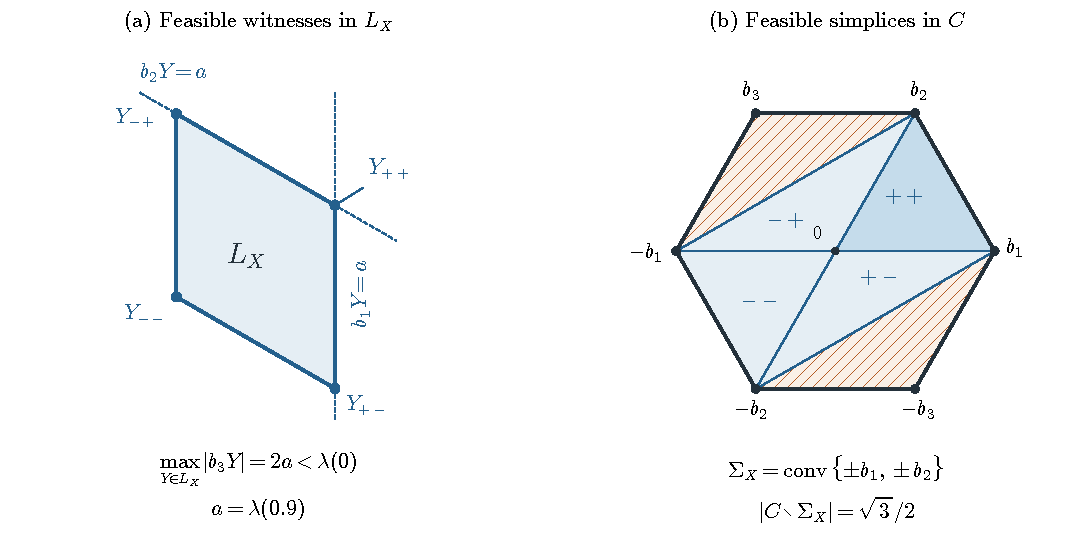
\includegraphics[width=\textwidth]{figures/feasible-simplex-deficit.pdf}
\caption{A feasible-simplex union can leave part of the polar uncovered.
Here $b_1=(1,0)$, $b_2=(1/2,\sqrt3/2)$,
$b_3=(-1/2,\sqrt3/2)$, $C=\operatorname{conv}\{\pm b_1,\pm b_2,\pm b_3\}$,
and $X=0.9(1,1/\sqrt3)$.
The third strip is redundant in $L_X$, as verified above. The four witnesses
$Y_{\epsilon_1\epsilon_2}$, defined by
$b_iY=\epsilon_i a$ for $i=1,2$, correspond to the four triangles
$\operatorname{conv}(0,\epsilon_1b_1,\epsilon_2b_2)$ with matching sign
labels. Their union is $\Sigma_X=\operatorname{conv}\{\pm b_1,\pm b_2\}$.
The two hatched caps have total area $\sqrt3/2$, one third of $|C|$.}
\label{fig:feasible-simplex-deficit}
\end{figure}

\subsection{Approximation of an arbitrary convex body}

\begin{corollary}[The symmetric volume-product inequality]
\label{cor:symmetric-inequality}
For every origin-symmetric convex body $K\subset\R^d$, $d\geq1$,
\[
 |K|\,|K^\circ|\geq\frac{4^d}{d!}.
\]
\end{corollary}

\begin{proof}
Put $Q=K^\circ$ and choose $a>0$ with $aB_2^d\subset Q$,
where $B_2^d$ is the Euclidean unit ball.
For $\varepsilon_j\downarrow0$, take a finite $\varepsilon_j$-net in
$Q$, adjoin its negatives, and let $Q_j$ be its convex hull. Thus
$Q_j\subset Q$, and their support functions satisfy, for every Euclidean
unit vector $u$,
\[
 h_Q(u)-\varepsilon_j\leq h_{Q_j}(u)\leq h_Q(u),
 \qquad h_Q(u)\geq a.
\]
For $\delta_j=\varepsilon_j/a<1$, this implies
\begin{equation}\label{eq:polar-approximation}
 (1-\delta_j)Q\subset Q_j\subset Q,
 \qquad
 K\subset A_j:=Q_j^\circ\subset(1-\delta_j)^{-1}K.
\end{equation}
The first inclusions follow from the support-function inequalities and
convex separation; the second follow by polarity. In particular $Q_j$
and $A_j$ are full-dimensional symmetric polytopes for large $j$.

Choose one vertex from each antipodal vertex pair of $Q_j$ as a row
list. These rows are nonzero and span. They are pairwise
nonproportional: two distinct boundary vertices on the same ray from
an interior origin cannot both be extreme, and the antipodal duplication
has already been removed. Their strip body is $A_j$.
Proposition~\ref{prop:simplex-integral} therefore gives
$|A_j|\,|Q_j|\geq4^d/d!$.
The homothetic bounds \eqref{eq:polar-approximation} show both
$|Q_j|\to|Q|$ and $|A_j|\to|K|$, because dilation by $t>0$ multiplies
volume by $t^d$. Passing to the limit proves the assertion. No smoothness,
simplicity, or general-position assumption is imposed on $K$.
In dimension one the assertion can also be read directly:
$K=[-a,a]$ has polar $[-1/a,1/a]$ and product $4$.
\end{proof}
